\chapter{Analisi descrittiva} %\label{2cap:analisi_descrittiva}

\section{Introduzione}

In questo capitolo viene presentata l'analisi descrittiva dei dati energetici raccolti per il periodo 2024-2025. Verranno descritte le fasi di elaborazione e pulizia dei dati (ETL), l'analisi del mix di produzione per ogni paese europeo e lo studio della stagionalità e dei profili orari di produzione. Infine, verrà analizzata la correlazione tra i prezzi dell'energia e le diverse fonti di produzione, integrando l'analisi con una rappresentazione geografica dei prezzi medi.

\subsection{Librerie utilizzate}

L'analisi è stata condotta utilizzando il linguaggio Python all'interno di un ambiente notebook, avvalendosi delle seguenti librerie:

\begin{itemize}
    \item \textbf{Pandas}: per la manipolazione e l'analisi dei dati in formato tabellare.
    \item \textbf{NumPy}: per il supporto a calcoli numerici e operazioni su array.
    \item \textbf{Matplotlib}: per la generazione di grafici e visualizzazioni statiche.
    \item \textbf{Seaborn}: per la creazione di visualizzazioni statistiche avanzate, come le heatmap di correlazione.
    \item \textbf{GeoPandas}: per la gestione di dati geospaziali e la realizzazione della mappa coropletica dell'Europa.
\end{itemize}

I dati sono stati pre-elaborati tramite la fase di ETL, descritta in modo approfondito al Capitolo~\ref{cap:dataset}.

\newpage

\section{Analisi del mix produttivo e distribuzione delle fonti energetiche}

La Dashboard di analisi del mix energetico, mostrata in Figura~\ref{fig:mix_produzione}, analizza lo scenario complessivo della generazione elettrica nei paesi europei monitorati, focalizzandosi sulla relazione tra distribuzione territoriale, tipologia di risorsa e specializzazione tecnologica dei singoli sistemi nazionali. 

Il sistema di visualizzazione è articolato in una matrice di sotto-grafici a barre (subplot) che scompone la produzione totale in dieci fonti energetiche fondamentali: Solare, Eolico Onshore, Eolico Offshore, Idroelettrico, Nucleare, Gas Fossile, Carbone, Lignite, Biomasse e Rifiuti. Per garantire una resa visiva immediata e una rigorosa coerenza interpretativa, sono state applicate specifiche regole di visualizzazione e formattazione:
\begin{itemize}
    \item \textbf{Codifica cromatica standardizzata:} a ciascuna delle dieci fonti energetiche è associato un colore univoco e distintivo, mantenuto inalterato in tutte le componenti della dashboard per favorire il tracciamento visivo;
    \item \textbf{Normalizzazione delle quote (\%):} per ogni paese, la quota di ciascuna fonte è calcolata rispetto alla somma delle dieci fonti selezionate. Le percentuali descrivono quindi la composizione relativa a queste fonti e non la quota sul totale di tutte le tecnologie di generazione;
    \item \textbf{Ordinamento decrescente strutturato:} all'interno di ciascun pannello, i paesi sono disposti in ordine decrescente in base al peso della specifica fonte, mettendo istantaneamente in risalto i mercati leader.
\end{itemize}

Accanto alla visione d'insieme, la dashboard permette di profilare l'impronta tecnologica dei singoli stati e di identificare le gerarchie di generazione. Questo approccio consente di distinguere nettamente le economie ancorate a un carico di base (\textit{baseload}) decarbonizzato o programmabile (come la prevalenza del nucleare in Francia o dell'idroelettrico nei paesi nordici) dai contesti caratterizzati da un'elevata penetrazione di fonti rinnovabili non programmabili o da una forte dipendenza dal gas di bilanciamento.

\begin{figure}[ht!]
    \centering
    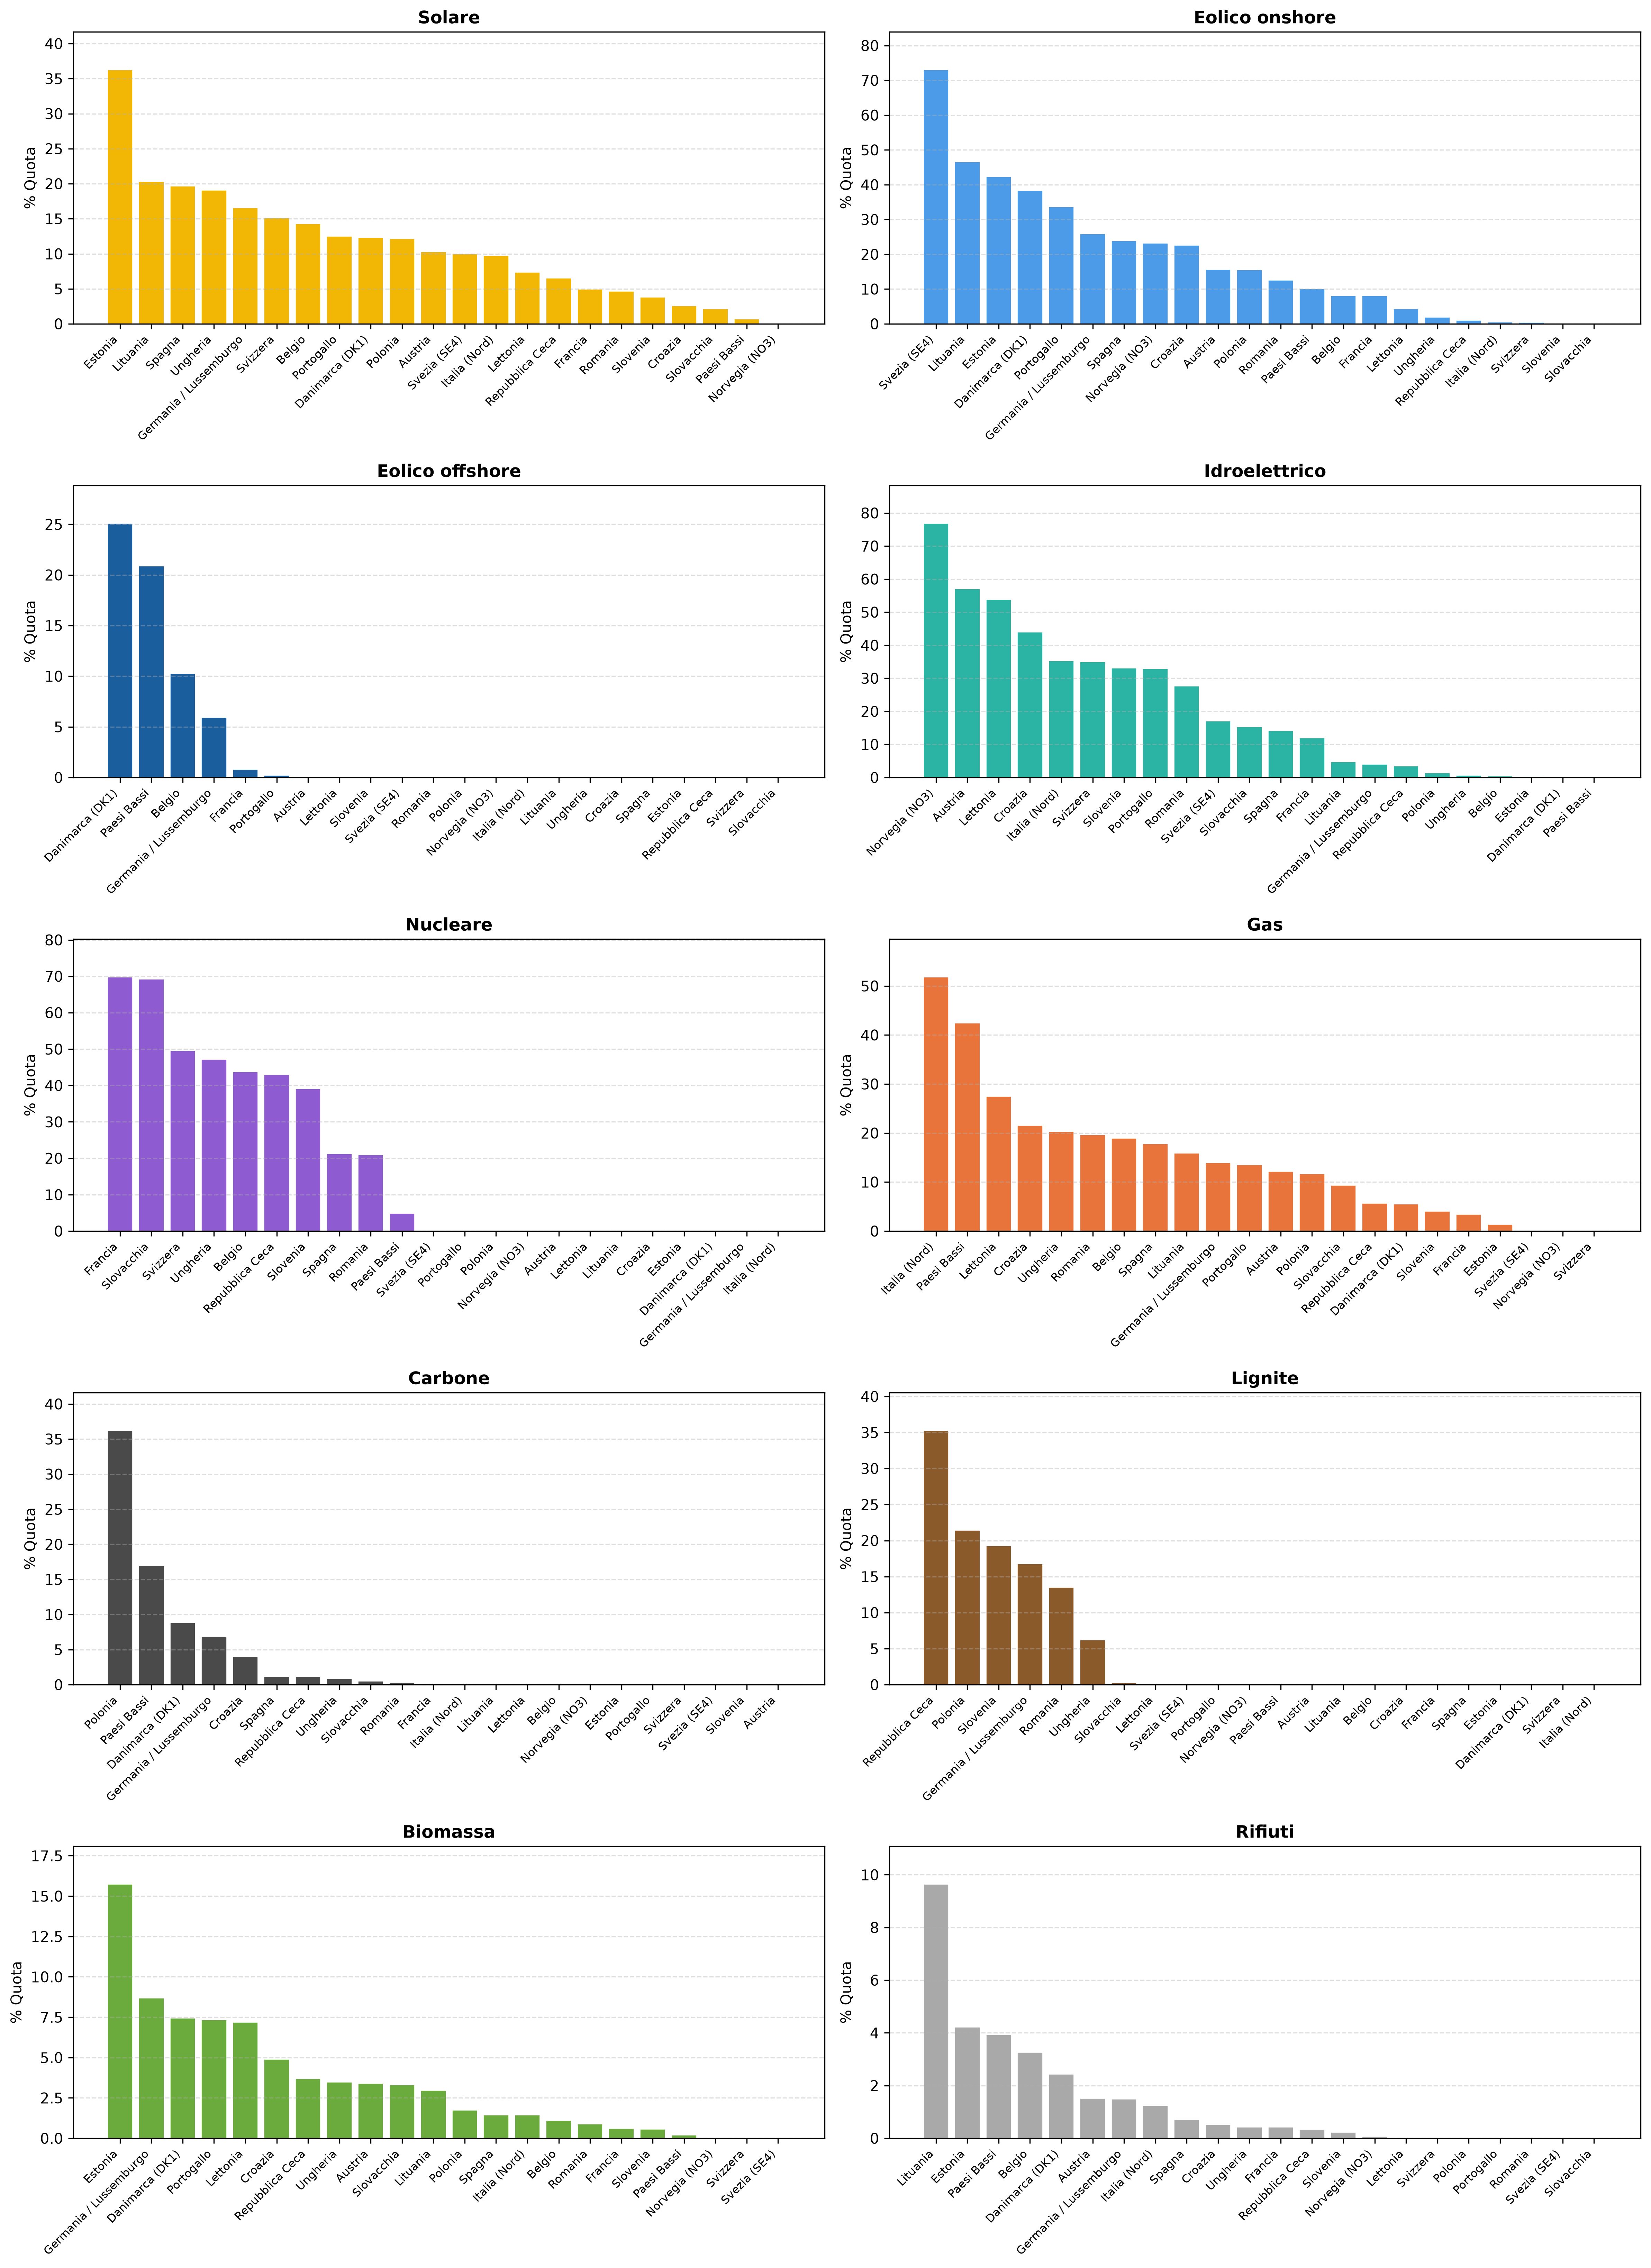
\includegraphics[width=\textwidth]{images/analisi/mix_produzione_fonti_separate.png}
    \caption{Distribuzione percentuale del mix produttivo energetico per paese e fonte.}
    \label{fig:mix_produzione}
\end{figure}

\newpage

\section{Analisi spaziale e distribuzione geografica dei prezzi dell'energia}

La Dashboard geografica dei prezzi medi, mostrata in Figura~\ref{fig:mappa_prezzi}, analizza lo scenario spaziale del mercato elettrico europeo, focalizzandosi sull'identificazione dei divari regionali, dei cluster di prezzo e della relazione tra posizione geografica e costo finale dell'energia.

La visualizzazione principale è costituita da una mappa a scala di colore ad alta risoluzione del continente europeo, costruita per mappare visivamente il prezzo medio spot (€/MWh) di ciascuna zona di mercato. Per garantire un'immediata comprensione delle dinamiche geografiche, il sistema adotta le seguenti specifiche metodologiche e visive:
\begin{itemize}
    \item \textbf{Proiezione cartografica europea:} utilizzo della proiezione su una cartina Europea, che preserva le proporzioni reali e le forme delle nazioni;
    \item \textbf{Scala cromatica continua a semaforo:} applicazione di una palette divergente invertita in cui il \textbf{Rosso} identifica gli \textit{hotspot} ad alto costo, il \textbf{Giallo} segnala i prezzi di fascia media e il \textbf{Verde} evidenzia le zone di mercato a basso costo;
    \item \textbf{Campitura dei dati mancanti:} utilizzo di una tonalità grigio chiaro neutra per identificare i territori extra-perimetro o non monitorati dal sistema ENTSO-E, evitando ambiguità interpretative.
\end{itemize}

Accanto alla rappresentazione estetica, la dashboard consente di evidenziare chiaramente i gradienti di prezzo tra i diversi contesti europei. L'analisi spaziale mette in luce una marcata spaccatura tra i mercati del Nord Europa (caratterizzati da prezzi medi contenuti grazie all'abbondanza di risorsa idroelettrica ed eolica) e le regioni del Centro-Sud Europa, dove la marginalità del gas fossile e i vincoli di interconnessione transfrontaliera mantengono il costo medio dell'elettricità su livelli strutturalmente più elevati.

\begin{figure}[ht!]
    \centering
    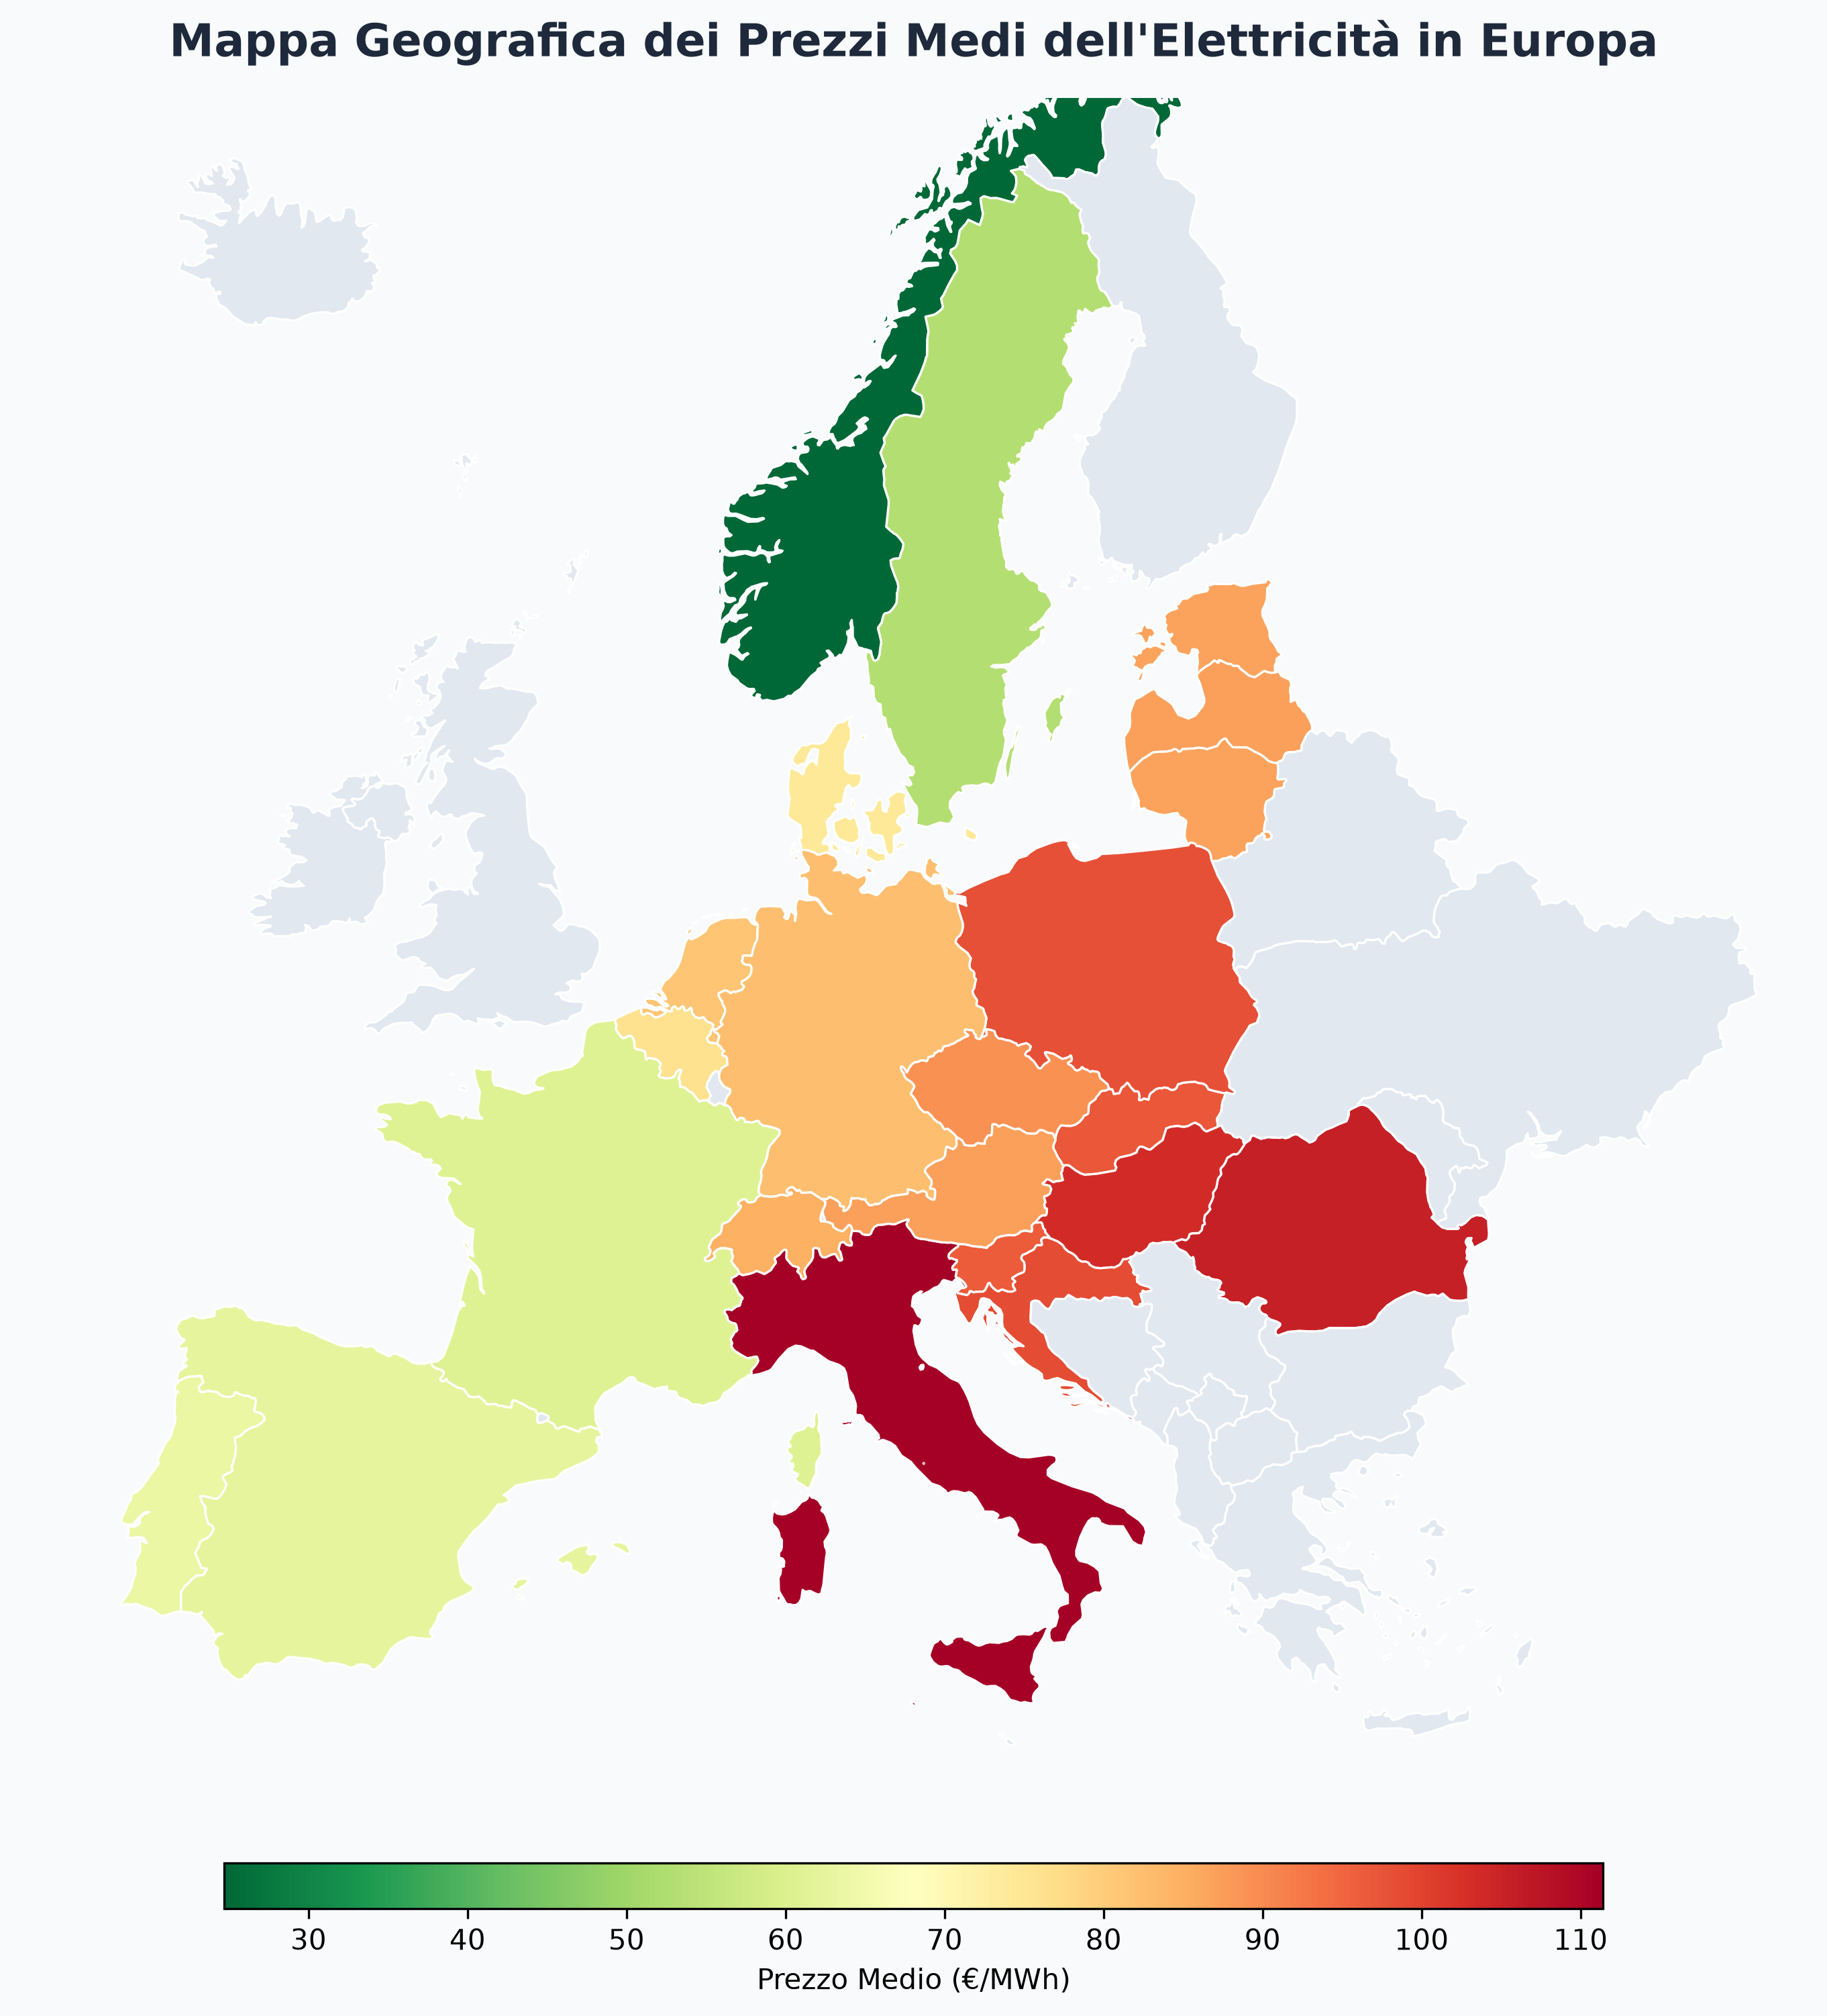
\includegraphics[width=0.56\textwidth]{images/analisi/mappa_geografica_prezzi_europa.png}
    \caption{Mappa coropletica della distribuzione geografica dei prezzi medi dell'energia in Europa (€/MWh).}
    \label{fig:mappa_prezzi}
\end{figure}

\section{Profilo orario medio della produzione}

\subsection{Profilo generale}

Per descrivere come varia la generazione elettrica nel corso della giornata, è stato calcolato il profilo orario medio delle dieci fonti considerate. Per ogni ora, da 0 a 23, il grafico riporta la produzione media osservata, espressa in MW. Nel profilo generale, aggregato sulle zone incluse nell'analisi, la fonte solare presenta il ciclo giornaliero più evidente: la produzione è prossima allo zero durante la notte, cresce nelle prime ore del mattino e raggiunge il massimo intorno alla tarda mattinata, per poi diminuire nel pomeriggio. Questo andamento è coerente con la disponibilità della radiazione solare.

Le altre fonti hanno profili medi differenti. Il nucleare rimane relativamente stabile durante le 24 ore; l'eolico onshore mostra variazioni più contenute rispetto al solare, mentre gas e idroelettrico presentano oscillazioni nel corso della giornata. Le fonti con produzione media più bassa appaiono quasi piatte sulla stessa scala verticale: ciò riflette soprattutto la differenza di ordine di grandezza rispetto alle fonti con valori medi più elevati. La media aggregata offre una visione d'insieme, ma può nascondere differenze tra i singoli paesi.

\begin{center}
    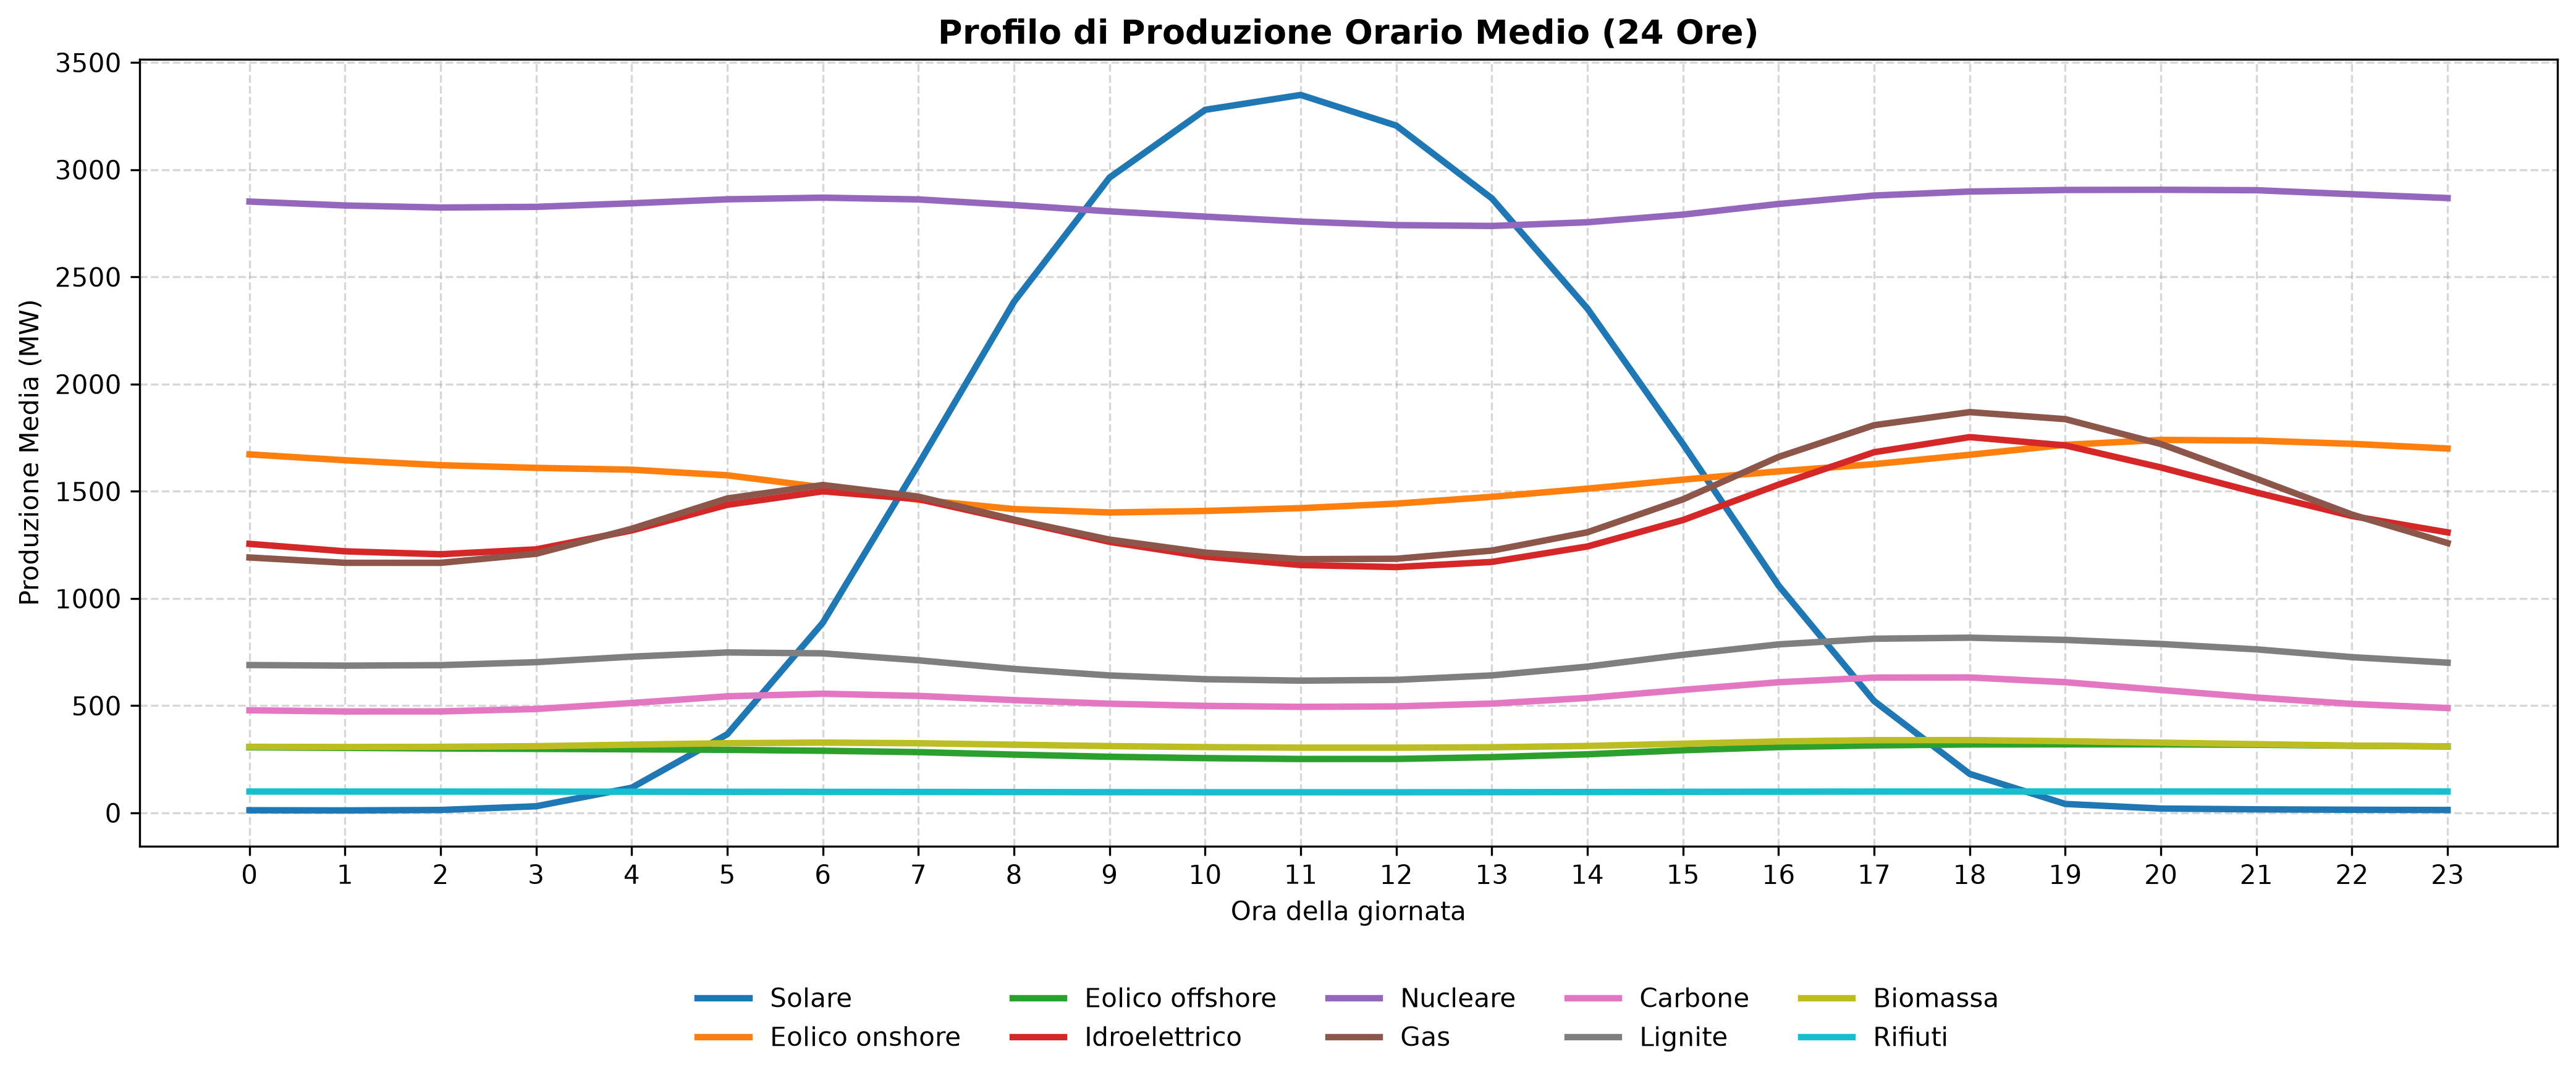
\includegraphics[width=\textwidth]{images/analisi/profilo_orario_medio.png}
    \captionof{figure}{Profilo orario medio della produzione per fonte, aggregato sulle zone considerate.}
    \label{fig:profilo_orario_medio}
\end{center}

\subsection{Profilo della zona IT\_NORD}

Nel dettaglio della zona italiana IT\_NORD, la produzione solare cresce rapidamente dopo le prime ore del mattino, raggiunge il massimo nelle ore centrali e torna su valori prossimi allo zero in serata. Il gas costituisce la fonte con la produzione media più alta nel profilo mostrato: diminuisce nelle ore centrali e aumenta nel tardo pomeriggio e in serata. L'idroelettrico varia in modo più graduale, con livelli medi rilevanti durante tutta la giornata e un incremento nelle ore pomeridiane.

Il profilo locale mette quindi in risalto il peso del gas e dell'idroelettrico nel sistema considerato, oltre alla concentrazione della produzione solare nelle ore di luce. Le altre fonti hanno valori medi molto inferiori e risultano compresse vicino alla base del grafico.
\begin{center}
    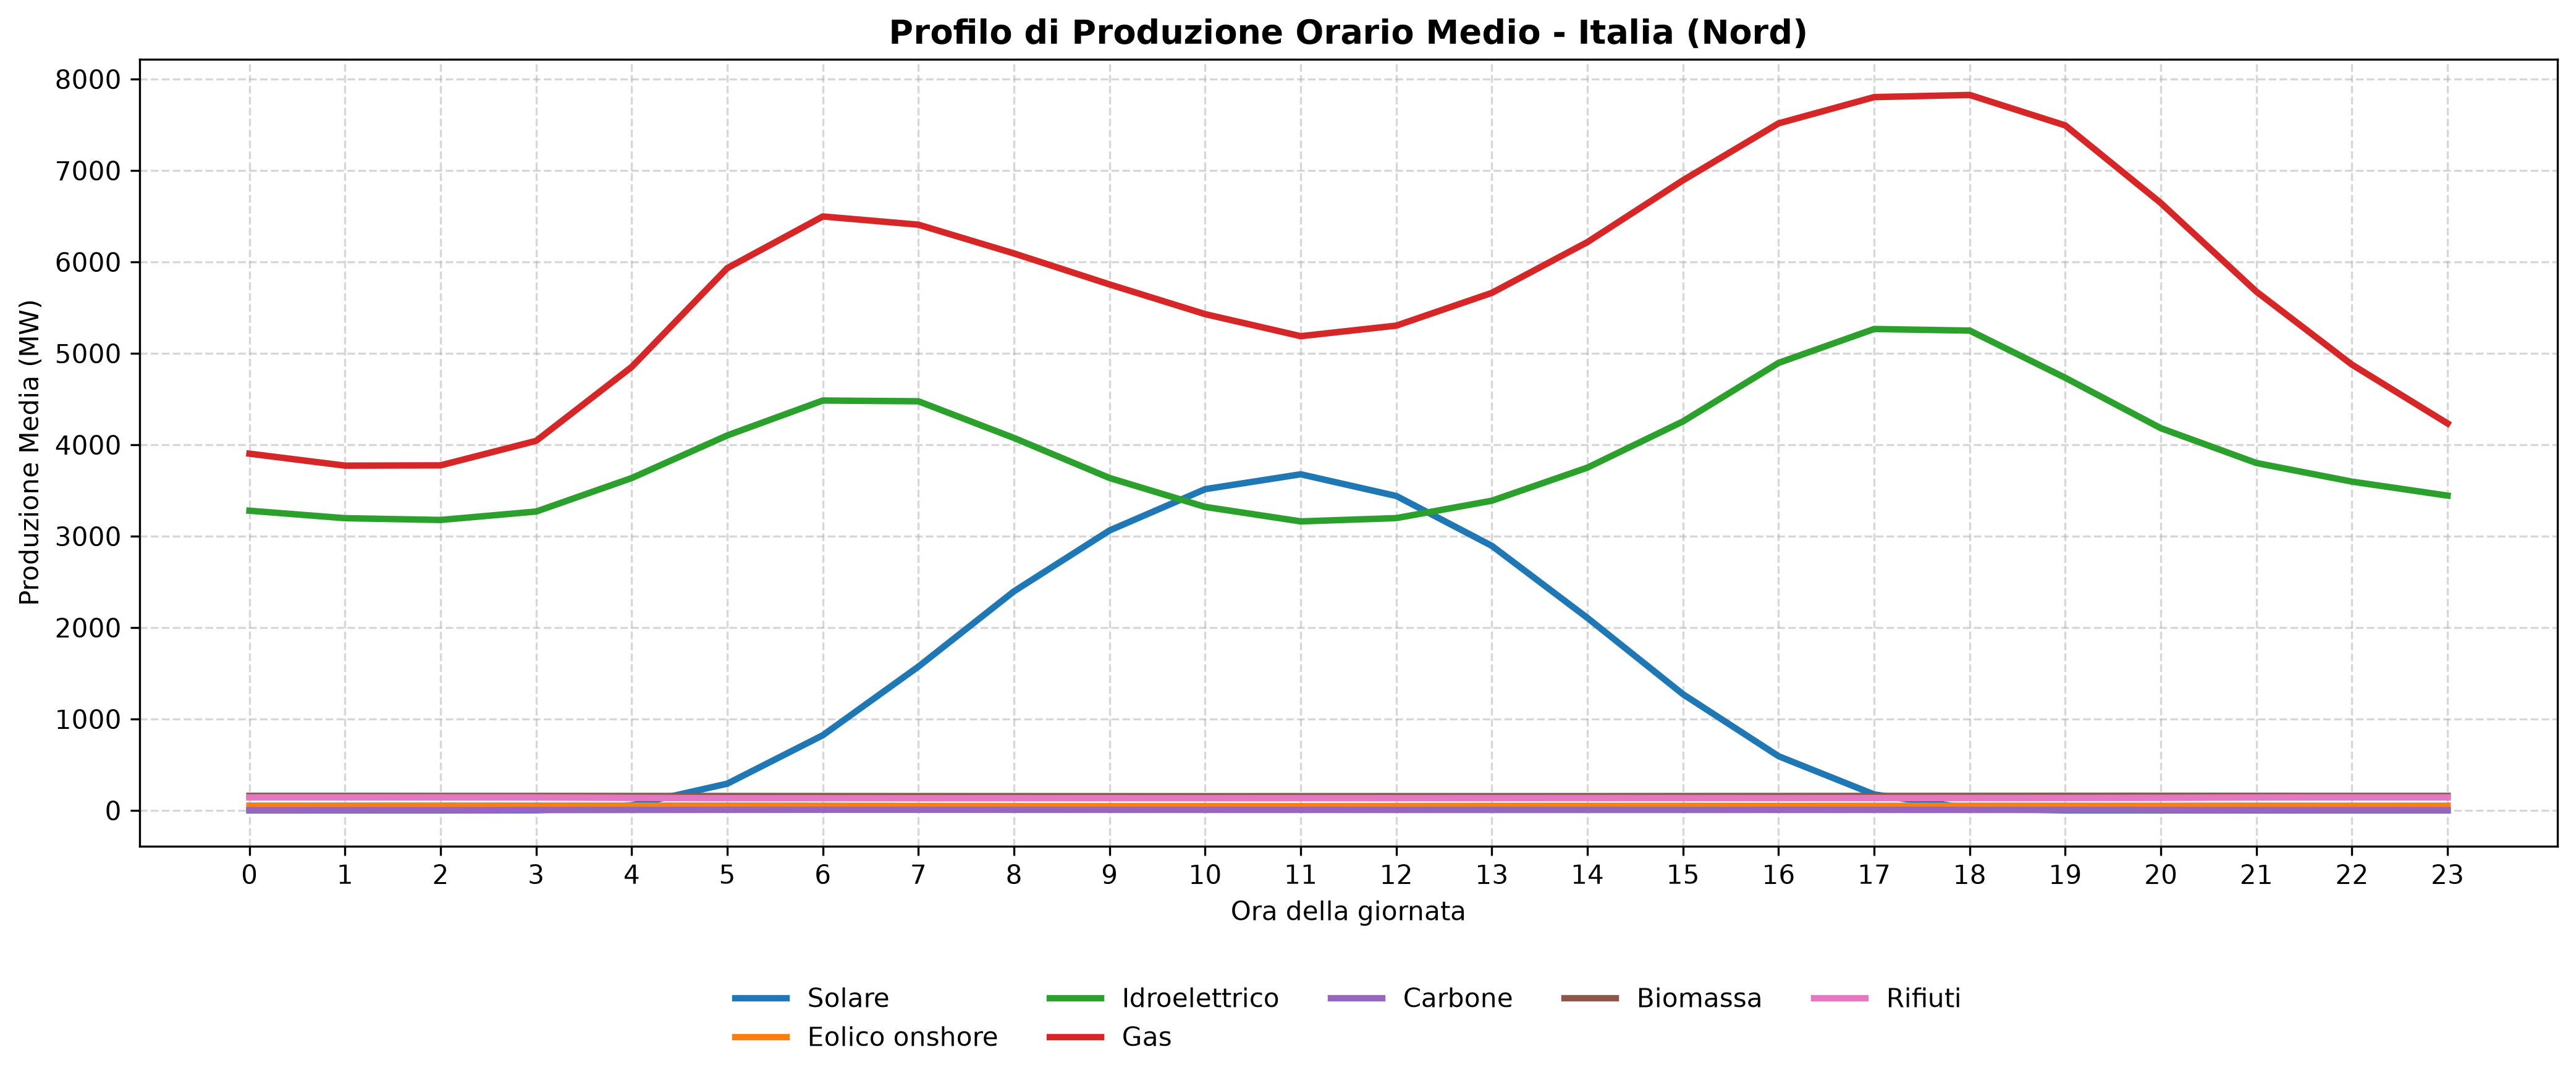
\includegraphics[width=\textwidth]{images/analisi/profilo_orario_IT_NORD.png}
    \captionof{figure}{Profilo orario medio della produzione per fonte nella zona di mercato IT\_NORD.}
    \label{fig:profilo_orario_it_nord}
\end{center}

\section{Stagionalità mensile della produzione}

\subsection{Andamento generale}

Per esaminare le variazioni nel corso dell'anno, la produzione è stata raggruppata per mese e ne è stata calcolata la media per ciascuna fonte. Nel profilo generale, il solare aumenta dall'inverno verso la primavera, raggiunge i valori medi massimi tra maggio e luglio e diminuisce in autunno. L'eolico onshore mostra invece valori più alti nei mesi invernali, una riduzione durante la primavera e l'estate e una nuova crescita verso la fine dell'anno. L'idroelettrico presenta variazioni meno regolari, mentre la produzione nucleare resta relativamente elevata e stabile, con un minimo nei mesi primaverili.

Gas, carbone e lignite mostrano andamenti mensili distinti: il gas diminuisce in primavera e risale soprattutto verso la fine dell'anno; carbone e lignite hanno oscillazioni più contenute nella media aggregata. Questi andamenti descrivono differenze tra le fonti, ma non ne identificano da soli le cause, che possono includere condizioni meteorologiche, domanda, disponibilità degli impianti e scambi tra zone.

\begin{center}
    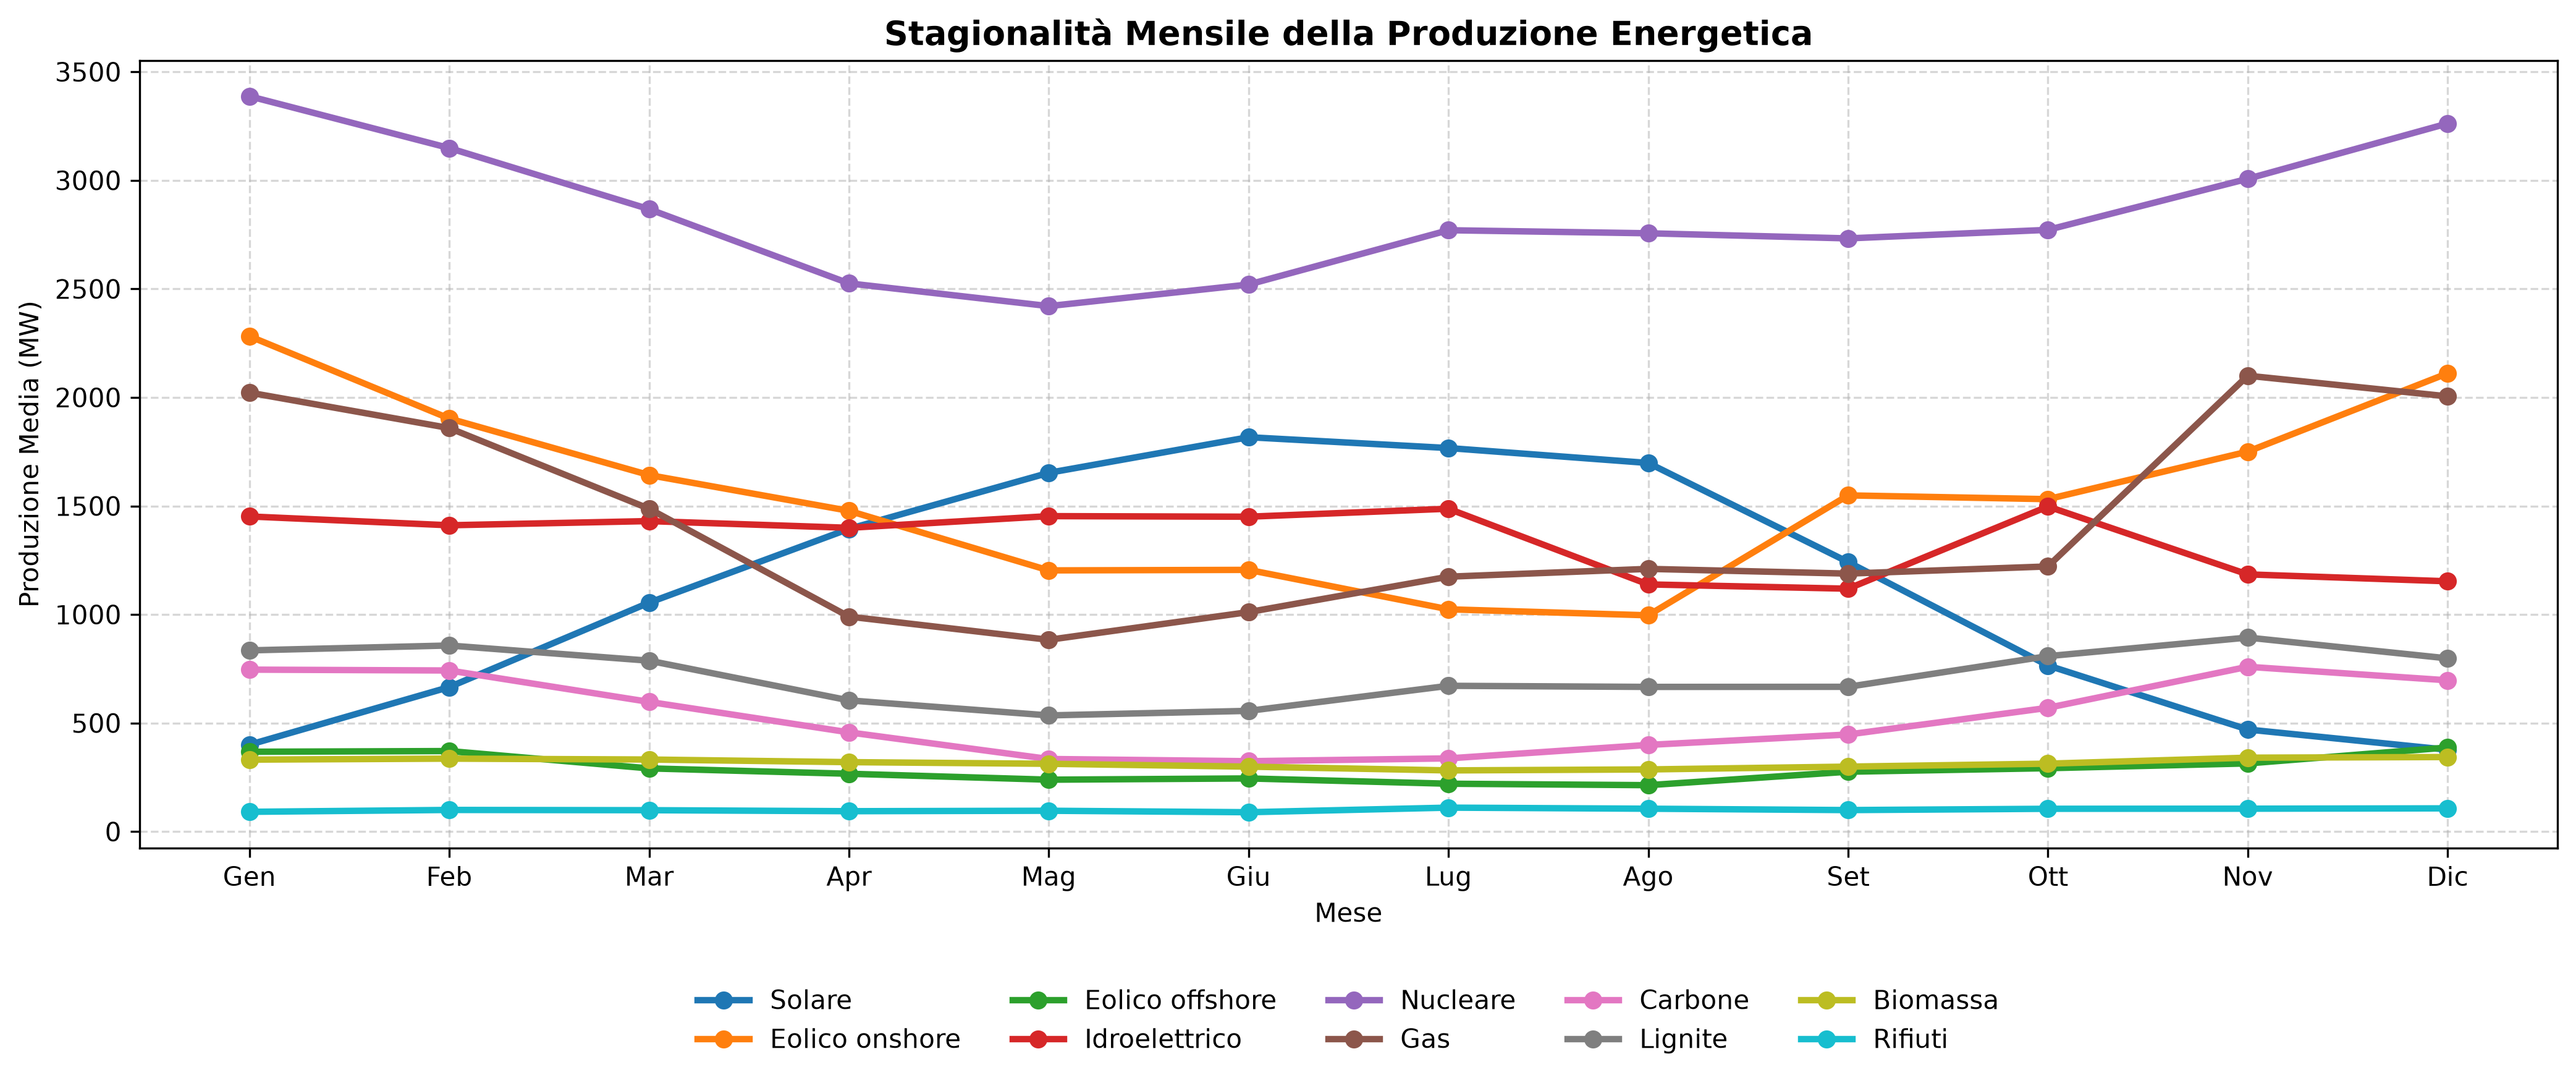
\includegraphics[width=\textwidth]{images/analisi/stagionalita_mensile.png}
    \captionof{figure}{Produzione media mensile per fonte, aggregata sulle zone considerate.}
    \label{fig:stagionalita_mensile}
\end{center}

\subsection{Andamento della zona IT\_NORD}

Per IT\_NORD, il solare raggiunge i valori medi più elevati tra maggio e luglio e diminuisce progressivamente nei mesi autunnali e invernali. L'idroelettrico cresce dalla primavera verso l'estate, raggiunge un massimo a luglio e poi cala in autunno. Il gas mantiene valori medi elevati nel corso dell'anno, con una marcata diminuzione in primavera e valori particolarmente alti in novembre e dicembre.

Il profilo locale evidenzia quindi fonti con andamenti stagionali diversi: il solare segue il ciclo della radiazione, l'idroelettrico raggiunge il massimo estivo nel periodo osservato e il gas aumenta nella parte finale dell'anno. Il grafico si riferisce al solo anno 2024, così da confrontare tutti i dodici mesi sulla base di un anno completo. L’andamento è descrittivo e non basta, da solo, a stabilire se la stagionalità osservata si ripeta negli anni successivi.

\begin{center}
    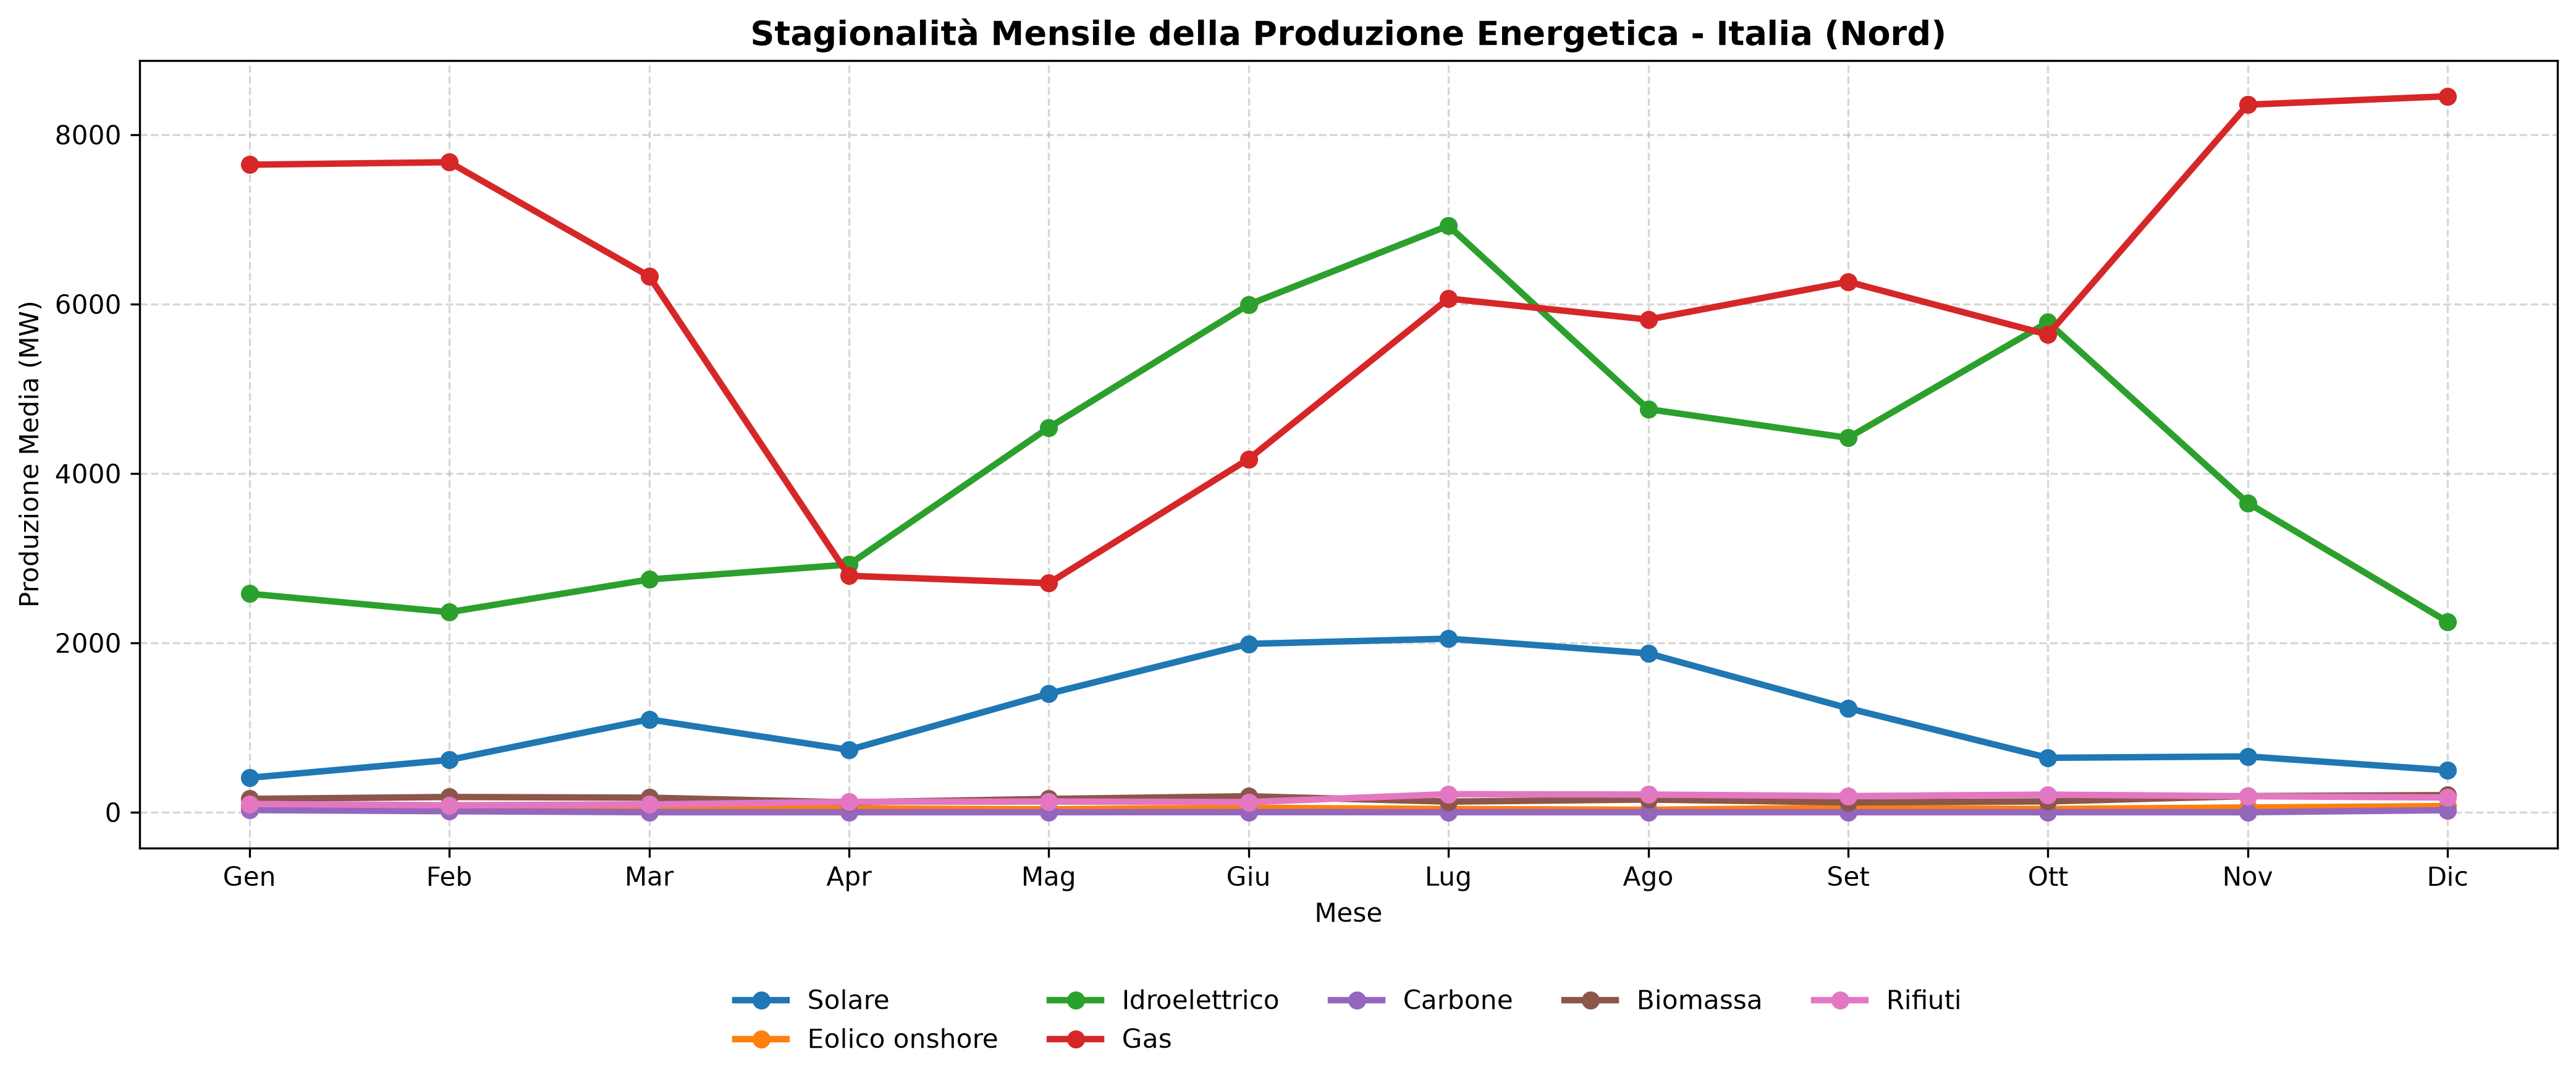
\includegraphics[width=\textwidth]{images/analisi/stagionalita_mensile_IT_NORD.png}
    \captionof{figure}{Produzione media mensile per fonte nella zona di mercato IT\_NORD.}
    \label{fig:stagionalita_mensile_it_nord}
\end{center}

\section{Matrice di correlazione di Pearson}

La matrice di Pearson misura la direzione e l'intensità dell'associazione lineare tra il prezzo dell'energia e la produzione delle diverse fonti, calcolandola separatamente per ciascun paese. I coefficienti variano tra $-1$ e $+1$:

\begin{itemize}
    \item valori positivi indicano che prezzo e produzione tendono a crescere insieme;
    \item valori negativi indicano che, quando una variabile cresce, l'altra tende a diminuire;
    \item valori prossimi a zero indicano una debole associazione lineare.
\end{itemize}

La Figura~\ref{fig:matrice_pearson_prezzo} riassume i coefficienti per i paesi e le fonti selezionati. Dalla matrice si osserva che:

\begin{itemize}
    \item la produzione solare presenta associazioni negative con il prezzo nella maggior parte delle zone;
    \item la produzione da gas presenta prevalentemente associazioni positive, con intensità variabile tra i mercati;
    \item le celle vuote indicano coefficienti non calcolabili, ad esempio quando una fonte non presenta variazione o dati validi sufficienti in una zona;
    \item le correlazioni descrivono associazioni e non dimostrano rapporti di causa-effetto: il prezzo dipende anche dalla domanda, dalla disponibilità degli impianti, dalle importazioni e da altri fattori.
\end{itemize}

\begin{center}
    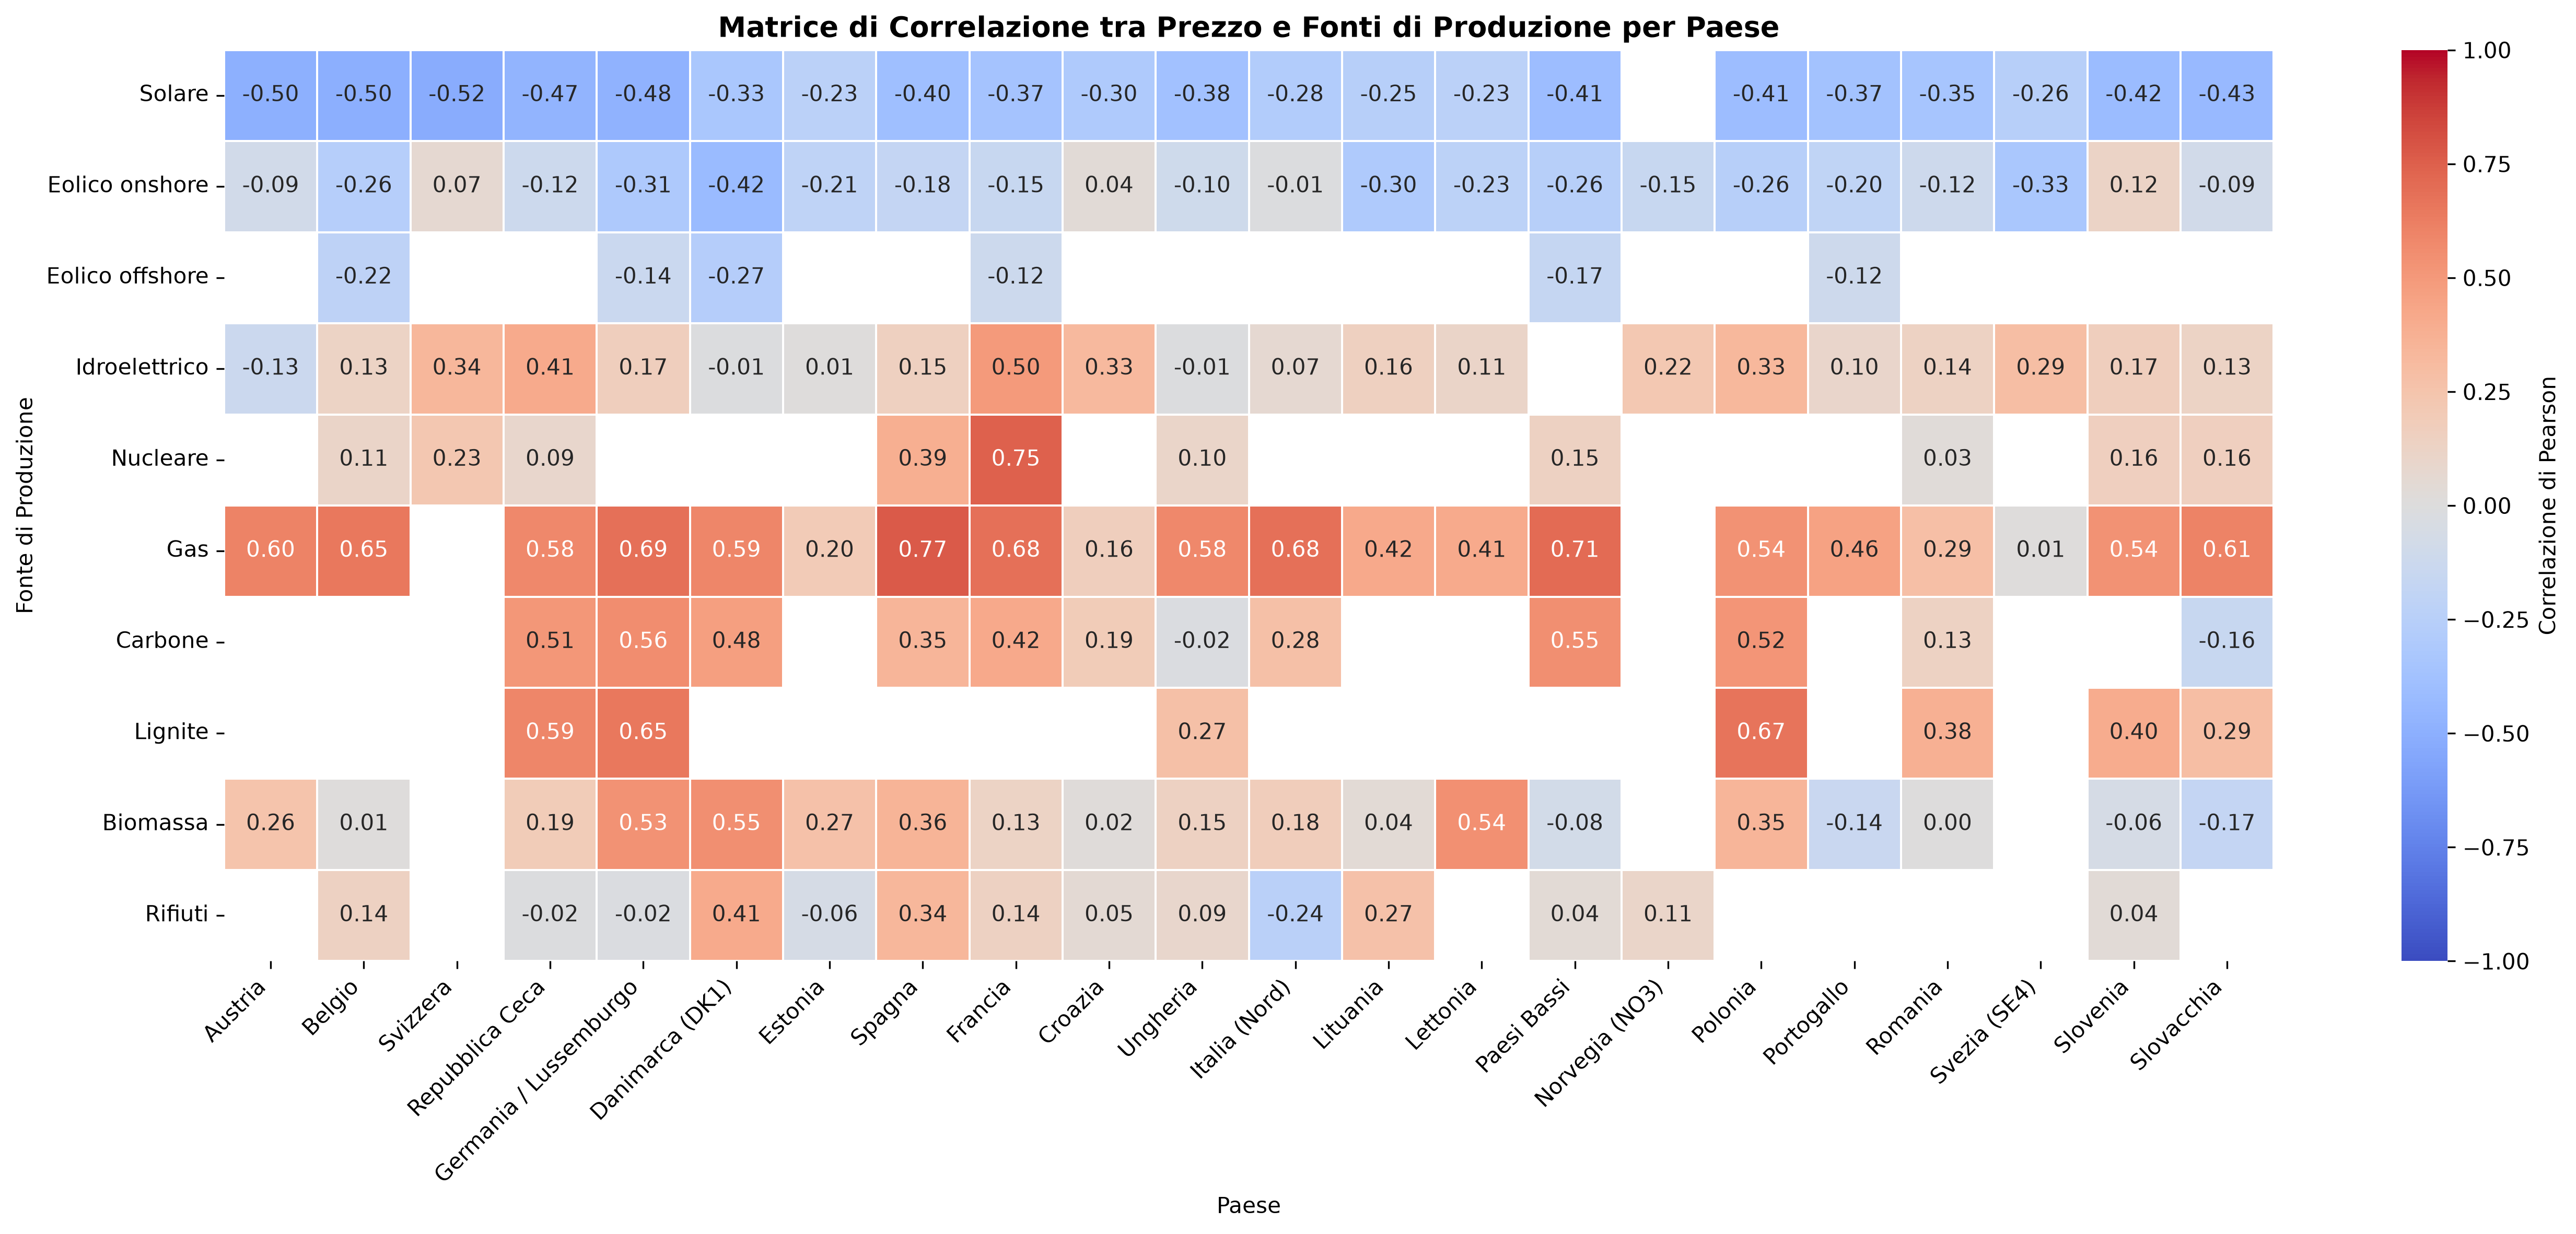
\includegraphics[width=0.95\textwidth]{images/analisi/matrice_correlazione_prezzo_paesi.png}
    \captionof{figure}{Matrice di correlazione di Pearson tra prezzo e produzione per paese.}
    \label{fig:matrice_pearson_prezzo}
\end{center}

\section{Matrice di correlazione di Spearman}

La correlazione di Spearman valuta l'associazione monotona tra due variabili sulla base dei loro ranghi. A differenza di Pearson, non richiede che la relazione sia lineare: è adatta a individuare situazioni in cui, al crescere di una variabile, l'altra tende generalmente a crescere o diminuire, anche con un andamento non proporzionale. Anche i coefficienti di Spearman variano tra $-1$ e $+1$ e la loro interpretazione riguarda associazione, non causalità.

La Figura~\ref{fig:matrice_spearman_prezzo} mostra che i pattern generali sono in parte simili a quelli di Pearson: la produzione solare presenta prevalentemente associazioni negative con il prezzo, mentre il gas mostra in molte zone associazioni positive. In diversi casi l'intensità dei coefficienti cambia rispetto a Pearson; ciò può indicare che l'associazione dipende dall'ordinamento dei valori e non segue una relazione perfettamente lineare. Le celle prive di valore rappresentano correlazioni non calcolabili per le stesse ragioni descritte nella matrice precedente.

\begin{center}
    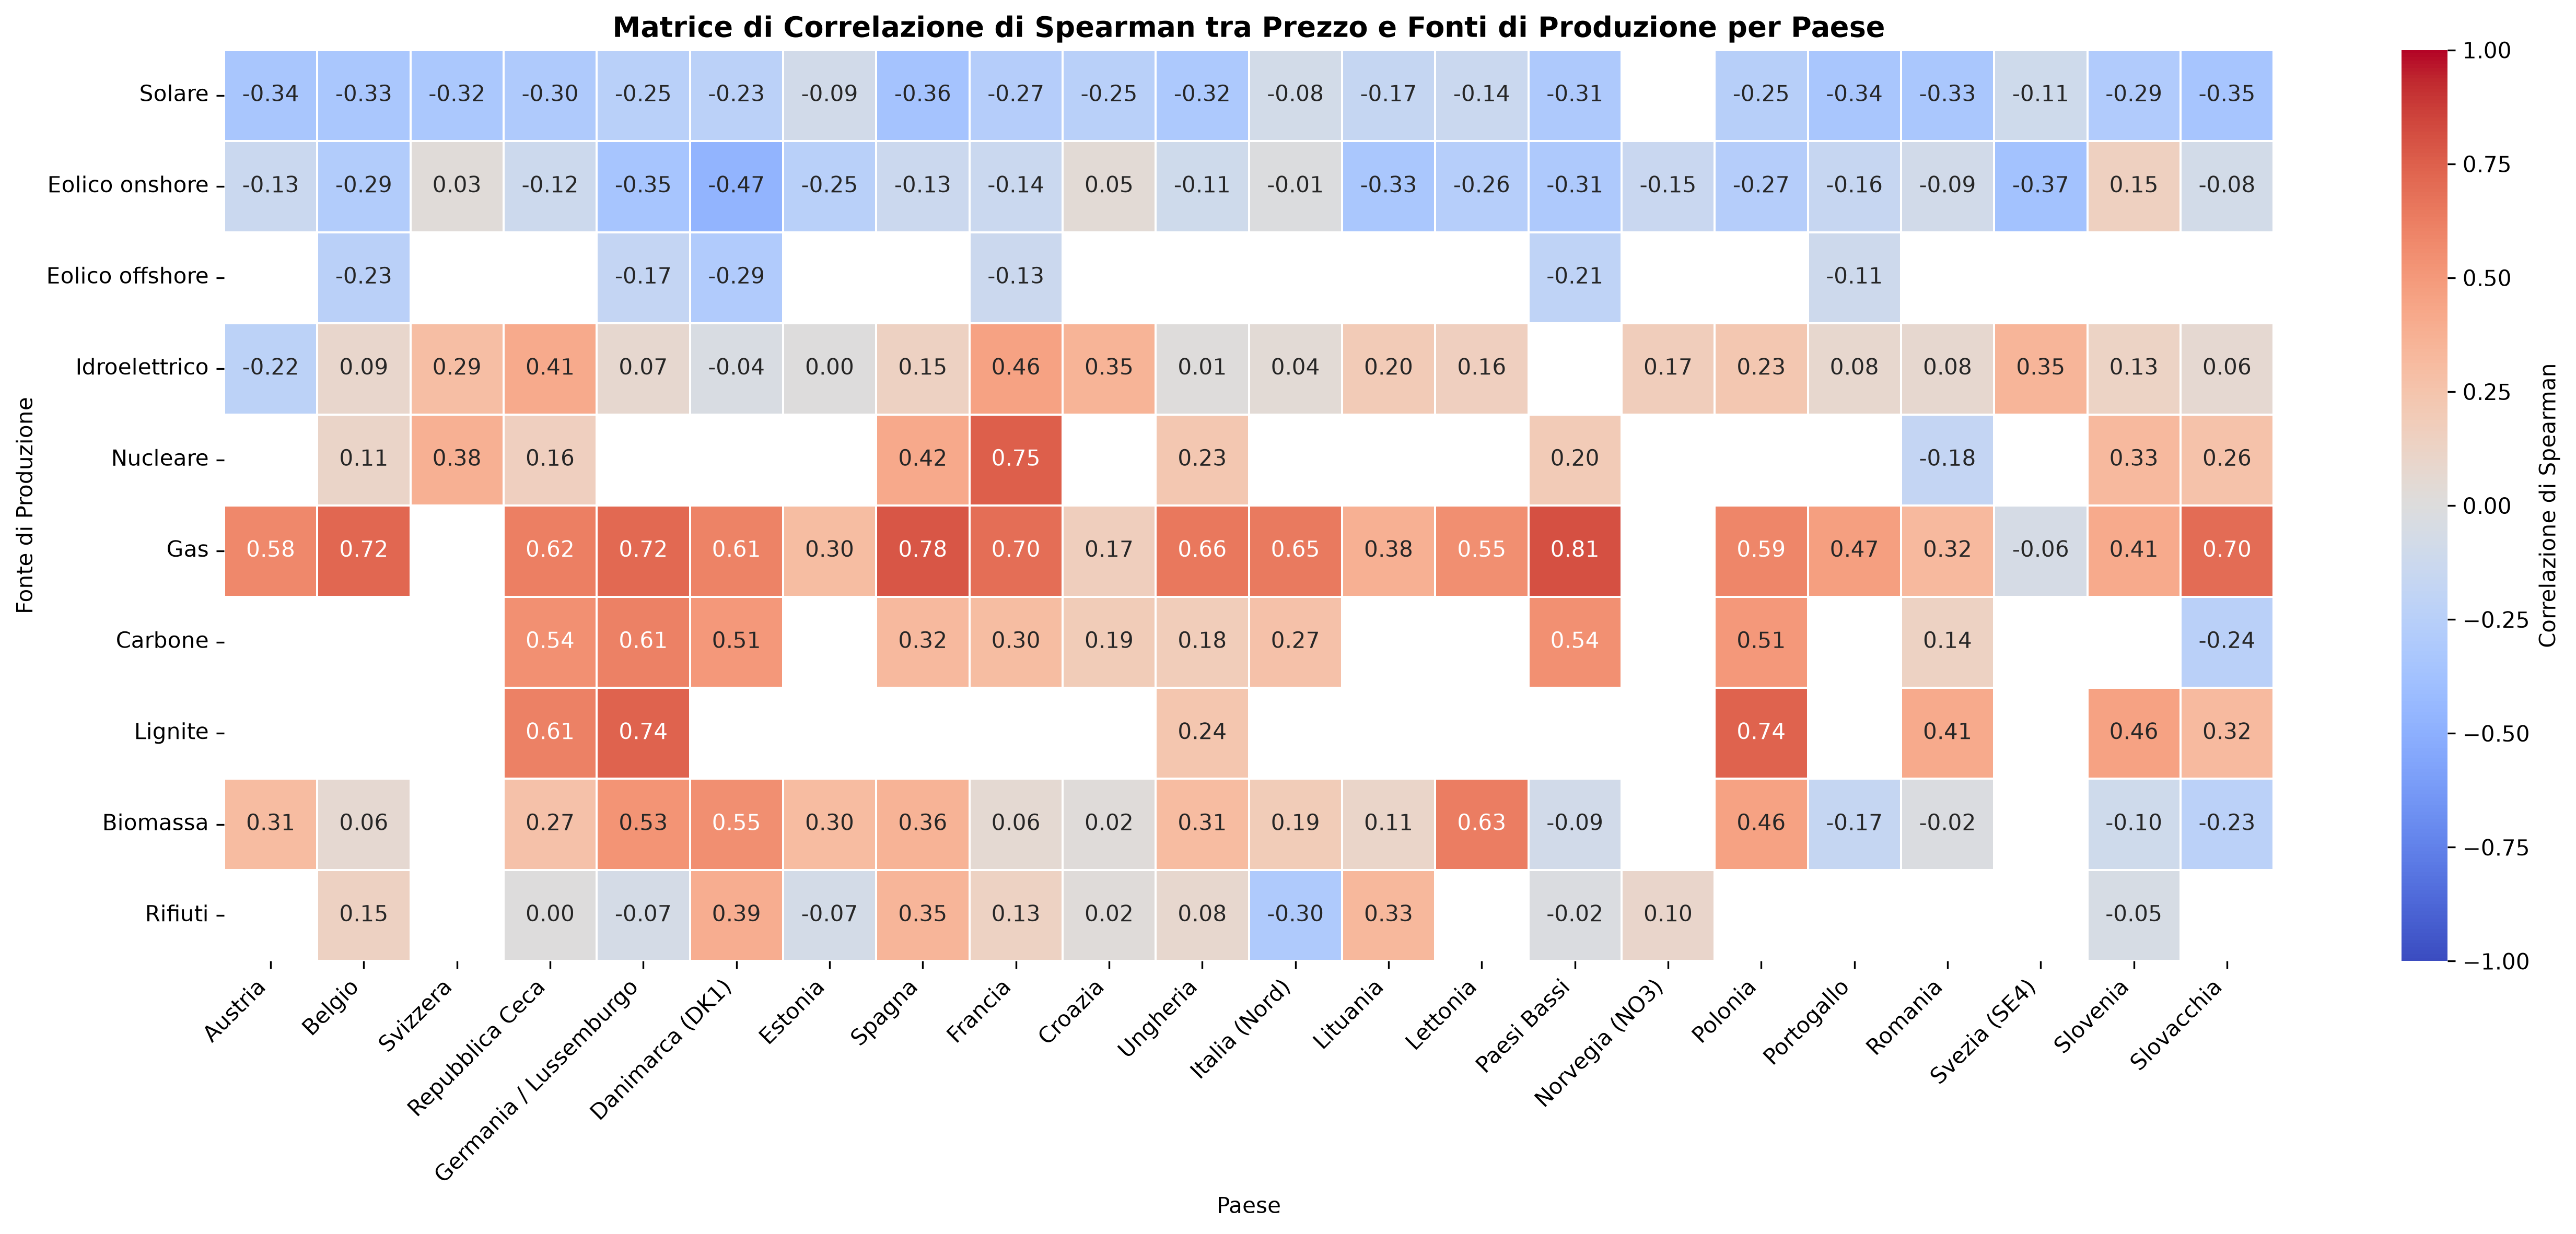
\includegraphics[width=0.95\textwidth]{images/analisi/matrice_spearman_prezzo_paesi.png}
    \captionof{figure}{Matrice di correlazione di Spearman tra prezzo e produzione per paese.}
    \label{fig:matrice_spearman_prezzo}
\end{center}
